\documentclass{article} % For LaTeX2e
\usepackage{iclr2027_conference,times}

\input{math_commands.tex}

\usepackage{hyperref}
\usepackage{url}
\usepackage{graphicx}
\usepackage{booktabs}
\usepackage{multirow}
\usepackage{amsmath}
\usepackage{amssymb}
\usepackage{xcolor}
\usepackage{enumitem}
\usepackage{caption}
\captionsetup{font=small}

\newcommand{\pifive}{$\pi_{0.5}$}
\newcommand{\occ}{\texttt{occluded}}
\newcommand{\cond}[1]{\texttt{#1}}

\title{Selective but Not Sufficient: Transcoder\\Circuit Analysis of Occlusion in a\\Vision-Language-Action Policy}

\author{Anonymous authors\\
Paper under double-blind review}

% \iclrfinalcopy % Uncomment for camera-ready version, but NOT for submission.

\begin{document}

\maketitle

\begin{abstract}
Vision-language-action (VLA) policies must act sensibly when a task-relevant object is hidden, yet nothing is known about how visibility is represented inside them and routed to actions. We present, to our knowledge, the first transcoder-based circuit analysis of a VLA policy. We train one TopK transcoder for each of the 18 layers of \pifive's Gemma language backbone and probe the model with a pixel-controlled occlusion protocol on LIBERO. Six simulator-rendered conditions separate occlusion from recoloring, removal and the mere appearance of an occluder, and a pre-registered validity battery passes in full: clean edits, bit-exact determinism, signal above sampling noise, a working patching ceiling, and faithful transcoders. We find 72 occlusion-selective features (0.78\% of the dictionary) spread across all layers. Patching only these features into unoccluded inputs moves the action toward its occluded counterpart $6.9\times$ more than norm-matched random features and $5.9\times$ more than color-selective features, and the effect is concentrated on the hidden object's image tokens. Yet they close only 3.9\% of the action gap, against 40.1\% for all transcoder features and 65.5\% for full MLP outputs, and fail our pre-registered 10-point criterion. Occlusion in \pifive{} is therefore represented by selective features that are not sufficient: the causal signal is carried by a distributed set of non-selective MLP features. We also show that interventions on a single MLP layer in \pifive{} are capped at 6.5\% of the effect while full residual swaps reach 91.8\%, and argue that circuit claims about VLAs should be reported relative to the ceiling of the intervened site.
\end{abstract}

\section{Introduction}
\label{sec:intro}

Vision-language-action models map camera images and an instruction to low-level robot actions by fine-tuning a vision-language backbone with an action head \citep{brohan2023rt2,kim2024openvla,black2024pi0,pi2025pi05}. They now reach high success rates on manipulation benchmarks such as LIBERO \citep{liu2023libero}, but we understand little about \emph{how} scene structure reaches the action. A basic case is occlusion. When the object a task refers to is hidden, a policy must either act on where the object probably is or change its behavior. Either way, some internal state must register that the object is not visible.

Mechanistic interpretability offers tools to find such states. Sparse autoencoders (SAEs) decompose activations into sparse, often interpretable features \citep{bricken2023monosemanticity,cunningham2024sparse,gao2025scaling}. \emph{Transcoders} instead approximate the computation of an MLP layer with a sparse, wide replacement \citep{dunefsky2024transcoders}, which makes it possible to trace circuits of features across layers \citep{ameisen2025circuit,lindsey2025biology,marks2025sparse}. Several recent works open up VLAs with SAEs, linear probes, steering vectors, activation injection or attention knockout \citep{haon2025mechanistic,buurmeijer2026observing,swann2026sparse,grant2026features,jin2026event,shi2026vlatrace}. None of them uses transcoders or feature-level causal tracing through the MLP computation.

We ask three questions about \pifive{} \citep{pi2025pi05}, a flow-matching VLA built on PaliGemma \citep{beyer2024paligemma}:
(\textbf{Q1}) Does its language backbone contain sparse features that respond selectively to the target object being occluded, and not to generic visual change, recoloring, removal, or the appearance of an occluder elsewhere?
(\textbf{Q2}) Do those features cause the change in the predicted action?
(\textbf{Q3}) Does intervening on them change closed-loop success?
Before looking at any result we fixed a gated plan: validity checks must pass before Q1; Q2 must beat random and color controls by 10 percentage points before Q3 is attempted.

The answer to Q1 is yes and to Q2 is \emph{only weakly}. Selective features exist in every layer and move the action several times more than matched controls, but they explain about 4\% of the effect, and most of the MLP-mediated signal flows through features that are not occlusion-selective. By the plan's rule Q3 was therefore not run. Our contributions are:
\begin{itemize}[leftmargin=*,itemsep=1pt,topsep=2pt]
  \item \textbf{A transcoder analysis of a VLA.} To our knowledge, this is the first analysis of a VLA policy with per-layer transcoders. We validate the transcoders both by reconstruction and by a functional splice test measured on the action (\S\ref{sec:tc}).
  \item \textbf{A controlled occlusion protocol with a validity battery.} Six pixel-exact conditions rendered from simulator segmentation isolate occlusion from appearance change, absence and occluder appearance. Five pre-registered checks certify the measurement before any feature claim (\S\ref{sec:protocol}, \S\ref{sec:validity}).
  \item \textbf{A clean negative result.} Occlusion-selective features exist and are causal above chance, but they are not sufficient. The effect is distributed across non-selective MLP features (\S\ref{sec:results}).
  \item \textbf{A methodological point for VLA circuit work.} In \pifive{} a single layer's MLP carries at most 6.5\% of the occlusion effect, while its full residual stream carries up to 91.8\%. Absolute effect thresholds at a single site can therefore be unreachable by construction, so we report effects relative to each site's own ceiling (\S\ref{sec:discussion}).
\end{itemize}

\section{Related work}
\label{sec:related}

\paragraph{Vision-language-action models.} RT-2 \citep{brohan2023rt2} and OpenVLA \citep{kim2024openvla} emit discretized actions from a VLM. $\pi_0$ \citep{black2024pi0} and \pifive{} \citep{pi2025pi05} couple a PaliGemma backbone (SigLIP \citep{zhai2023siglip} and Gemma \citep{gemma2024}) with an action expert trained by flow matching \citep{lipman2023flow}. The expert attends to the backbone's key/value cache of image, prompt and state tokens. We use the LeRobot port of \pifive{} \citep{cadene2024lerobot} fine-tuned on LIBERO \citep{liu2023libero}.

\paragraph{Sparse dictionaries and circuits.} SAEs recover sparse, interpretable directions in residual streams \citep{bricken2023monosemanticity,cunningham2024sparse}. TopK activations make them easy to train at scale \citep{gao2025scaling}. Transcoders reconstruct an MLP's \emph{output} from its \emph{input} through a sparse bottleneck. The result is an interpretable replacement of the layer's computation that supports input-invariant circuit analysis \citep{dunefsky2024transcoders}. Cross-layer transcoders and attribution graphs extend this to full circuit tracing in LLMs \citep{ameisen2025circuit,lindsey2025biology}, and sparse feature circuits identify small causal subgraphs \citep{marks2025sparse}. Concurrent work applies transcoders to a vision-language model to trace visual grounding \citep{damianos2026transcoders}. That study has no action head and no embodiment.

\paragraph{Causal interventions.} Activation patching swaps internal states between a clean and a corrupted run \citep{meng2022locating,wang2023interpretability}. Its outcome depends strongly on the metric, the corruption and the site \citep{zhang2024towards,heimersheim2024patching}, and subspace patching can create illusory effects \citep{makelov2024subspace}. We therefore pair every feature patch with norm-matched random and semantically matched (color) controls, and report the patch's ceiling at the same site.

\paragraph{Interpretability of VLAs.} Prior work does not use transcoders or feature circuits:
\begin{itemize}[leftmargin=*,itemsep=0pt,topsep=1pt]
  \item \citet{haon2025mechanistic} project feed-forward activations of $\pi_0$ and OpenVLA onto token embeddings and steer behavior.
  \item \citet{buurmeijer2026observing} define feature observability and controllability with linear probes and optimal-control interventions on \pifive{} and OpenVLA.
  \item SAEs on VLAs reveal steerable motion and semantic features \citep{swann2026sparse}, which can be grounded to behavioral events \citep{jin2026event}.
  \item \citet{grant2026features} use activation injection, SAEs and probes across six VLAs, including \pifive{}, and find that vision pathways dominate action generation.
  \item VLA-Trace \citep{shi2026vlatrace} combines CKA, attention knockout and behavioral probes on \pifive{} and OpenVLA over LIBERO, reporting narrow visual bottlenecks in \pifive{}.
  \item \citet{zhang2026embodied} estimate visual attribution by interventional masking.
\end{itemize}
Our work adds MLP-level sparse replacements, feature-selective patching with matched controls, and a targeted question about occlusion.

\section{Method}
\label{sec:method}

\subsection{Model and intervention sites}
\pifive{} embeds each camera image into 256 SigLIP tokens and the prompt together with the discretized proprioceptive state into up to 200 language tokens. It processes this \emph{prefix} with bidirectional attention through an 18-layer Gemma-2B decoder. A 300M-parameter action expert then integrates a 50-step action chunk with 10 Euler steps of flow matching, attending at every layer to the prefix key/value cache. All interventions act on the prefix pass, so they change every key and value the expert reads. For decoder layer $\ell$ we hook the MLP input $\vx_\ell$ (the post-attention RMSNorm output), the MLP output $\vy_\ell$, and the layer's residual output $\vh_\ell$, at every valid prefix token. Padding tokens and the empty third camera slot are masked out.

\subsection{Controlled occlusion protocol}
\label{sec:protocol}
We replay LIBERO demonstrations and render, at a chosen time step, six versions of both camera images (Figure~\ref{fig:protocol}). All are edited in pixel space from a MuJoCo segmentation mask $M$ of the target object:
\begin{itemize}[leftmargin=*,itemsep=0pt,topsep=1pt]
  \item \cond{base}: the unedited render.
  \item \cond{recolor}: pixels in $M$ shaded red, preserving luminance.
  \item \cond{absent}: the object moved out of the scene and re-rendered, composited inside $M$ dilated by 6\,px so its shadow disappears too.
  \item \occ{}: $M$ dilated by 2\,px and filled with flat gray.
  \item \cond{slab\_miss}: the same gray shape translated off the object and away from the robot.
  \item \cond{occluded\_absent}: \cond{absent} with the same gray paint.
\end{itemize}
Robot state, prompt and sampling noise are identical across conditions. Each edit may change pixels only inside its declared region.

\begin{figure}[t]
  \centering
  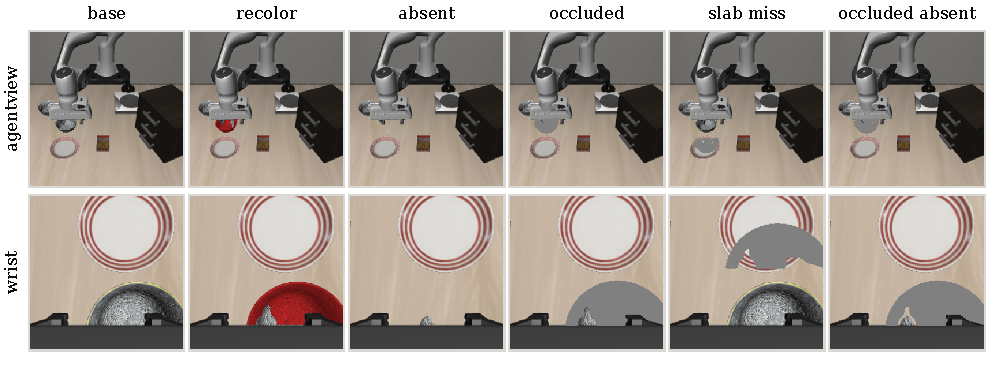
\includegraphics[width=\linewidth]{figures/fig_protocol.pdf}
  \caption{\textbf{Controlled occlusion protocol}, probe frame 0 (LIBERO-Spatial task 0, demonstration 0, $t{=}35$), shown as the policy sees it. The target bowl is edited in both cameras. The target occupies 0.5--1.2\% of the agentview image but 4--20\% of the wrist image across frames.}
  \label{fig:protocol}
\end{figure}

\paragraph{Action-gap metric.} For a frame with fixed noise, let $\va_c\in\R^{50\times7}$ be the normalized action chunk under condition $c$. The \emph{gap} is $g=\mathrm{RMSE}(\va_{\text{base}},\va_{\text{occ}})$. A patch applied to the base run (\emph{inject}) yields $\va'$, and we report
\begin{equation}
  \text{gap closed} \;=\; 100\left(1-\frac{\mathrm{RMSE}(\va',\va_{\text{occ}})}{g}\right)\%.
\end{equation}
The \emph{remove} direction patches the occluded run toward base analogously.

\subsection{Transcoders}
\label{sec:tc}
For each layer we train a TopK transcoder \citep{dunefsky2024transcoders,gao2025scaling}:
\begin{equation}
  \vf(\vx) = \mathrm{TopK}_k\!\left(\mathrm{ReLU}\!\left(\mW_{\text{enc}}\tfrac{\vx-\boldsymbol\mu_x}{s_x}+\vb_{\text{enc}}\right)\right),\qquad
  \hat\vy = s_y\!\left(\mW_{\text{dec}}^\top\vf(\vx)+\vb_{\text{dec}}\right)+\boldsymbol\mu_y,
\end{equation}
with 512 features, $k{=}16$ and unit-norm decoder rows $\vd_j$. The scalars $s_x,s_y$ normalize the mean-centered inputs and outputs to unit mean norm, so the training loss $\E\|\hat\vy_n-\vy_n\|^2$ equals the fraction of variance unexplained (FVU). An AuxK term ($k_{\text{aux}}{=}64$, weight $1/32$) revives dead features. We train with Adam (learning rate $2\times10^{-3}$, batch 1,024, 3,000 steps) on 26,852 valid prefix tokens from 47 forward passes: the 4 probe frames in 6 conditions, plus 23 unedited frames from the same demonstrations. A random 10\% of tokens is held out.

\subsection{Selecting occlusion features}
For feature $j$, let $A_{j}(c)$ be its activation summed over valid prefix tokens under condition $c$, and $\Delta_{j}(c)=A_j(c)-A_j(\text{base})$ per frame. A feature is \emph{occlusion-selective} if
(i) $\Delta_j(\occ)>0$ on every probe frame;
(ii) its specificity $1-\max_{c}\overline{|\Delta_j(c)|}\,/\,\overline{\Delta_j(\occ)}\ge0.5$ for $c\in\{\cond{recolor},\cond{absent},\cond{slab\_miss}\}$ (bars denote means over frames);
(iii) the rise $\overline{\Delta_j(\occ)}$ exceeds one typical token-level firing of the feature.
We keep at most 8 per layer, ranked by specificity $\times$ rise. A size-matched \emph{color} control set is ranked the same way with \cond{recolor} as the target.

\subsection{Causal patching and controls}
To set a feature set $S$ to its values from a target run, we edit the MLP output as
\begin{equation}
  \vy'_\ell = \vy_\ell + s_y\sum_{j\in S}\left(f_j^{\text{tgt}}-f_j(\vx_\ell)\right)\vd_j ,
\end{equation}
which leaves the transcoder's reconstruction error in place. The controls are:
\begin{itemize}[leftmargin=*,itemsep=0pt,topsep=1pt]
  \item \emph{random, same norm}: 5 random sets of $|S|$ features, rescaled per token to the norm of the $S$ edit;
  \item \emph{random, raw}: the same random sets, unscaled;
  \item \emph{color}: the color-selective set;
  \item \emph{all transcoder features};
  \item \emph{MLP swap}: $\vy_\ell\leftarrow\vy_\ell^{\text{occ}}$, the ceiling of any intervention at this site;
  \item \emph{full swap}: $\vh_\ell\leftarrow\vh_\ell^{\text{occ}}$.
\end{itemize}
Patches are applied to all valid tokens, only to the target's image tokens (patches that are at least 10\% covered by paint), or to all other tokens. We patch the three top-scoring layers individually, the three jointly, and \emph{all 18 layers jointly}.

\section{Experimental setup}
\label{sec:setup}
\paragraph{Policy and task.} We use \texttt{lerobot/pi05\_libero\_finetuned} in bfloat16 (LeRobot 0.6.1). Model compilation is disabled so that hooks execute eagerly. The task is LIBERO-Spatial task 0, ``pick up the black bowl between the plate and the ramekin and place it on the plate''; the target is the bowl named in the task's BDDL goal, and a distractor bowl is present. Images are rendered at $256\times256$ from the agentview and wrist cameras.

\paragraph{Probe frames.} We replay demonstrations 0 and 1 (98 and 84 steps; the bowl is lifted at $t{=}51$ and $t{=}47$). We score 8 evenly spaced pre-grasp candidates per demonstration by their base-vs-occluded gap and keep the two largest per demonstration: $t\in\{35,41\}$ and $\{5,32\}$. This choice maximizes signal (candidate gaps range 0.15--0.67), so the frames are not a random sample.

\paragraph{Pre-registered criteria.} The criteria were fixed before the run:
\begin{itemize}[leftmargin=*,itemsep=0pt,topsep=1pt]
  \item Check 3: the gap must be at least 0.02.
  \item Check 4: a full-layer swap must close at least 90\% of the gap at some layer.
  \item Check 5: median held-out FVU must be at most 0.20.
  \item Goal 2: the occlusion set must close at least 10 points more than both the same-norm random and the color control.
\end{itemize}
The whole pipeline takes about 30 minutes on one A100 GPU (Appendix~\ref{app:repro}).

\section{Results}
\label{sec:results}

\subsection{The measurement instrument is sound}
\label{sec:validity}
Table~\ref{tab:validity} summarizes the validity battery; all five checks pass.
\begin{itemize}[leftmargin=*,itemsep=1pt,topsep=2pt]
  \item \textbf{Clean, deterministic, real signal.} Edits change zero pixels outside their regions across 40 frame$\times$condition$\times$camera combinations, and repeated forward passes agree to the last bit. Occluding the bowl shifts the action chunk by 0.52--0.67 RMSE, 2.9--4.4$\times$ the shift caused by changing only the sampling noise. Removing the bowl shifts it more (0.83--1.06).
  \item \textbf{Where the signal lives.} Replacing the whole residual stream at layer $\ell$ with the occluded run's closes 91.8\% of the gap at $\ell{=}3$. Closure falls below 50\% from layer 9 and below 5\% from layer 14 (Figure~\ref{fig:layers}a). The occlusion information that the action expert uses is therefore present in the prefix by the early-to-middle layers.
  \item \textbf{A single MLP carries very little.} Swapping one layer's \emph{MLP output} closes only 0.0--6.5\%.
  \item \textbf{Faithful transcoders.} Median held-out FVU is 0.174 (range 0.018--0.258; all 512 features alive in every layer). Splicing any single transcoder into the model, without its error term, moves the action by at most 0.16 of the occlusion gap.
\end{itemize}
A first run with 400 training steps reached a median FVU of 0.209 and failed Check 5. We met the gate by training longer, not by relaxing the threshold.

\begin{table}[t]
\caption{\textbf{Pre-registered validity battery} (4 probe frames). All checks pass.}
\label{tab:validity}
\centering\small
\resizebox{\linewidth}{!}{%
\begin{tabular}{@{}lll@{}}
\toprule
Check & Criterion & Result \\
\midrule
1. Edits are clean & $<0.2\%$ changed pixels outside edit region & 0.000\% (40/40); state \& prompt identical \\
2. Determinism & repeated forward, max $|\Delta\va|=0$ & 0.0 on all frames \\
3. Signal exists & gap $\ge0.02$ & 0.516--0.666 (2.9--4.4$\times$ seed noise) \\
4. Ceiling works & full swap $\ge90\%$ at some layer & 91.8\% at layer 3 \\
5. Transcoders faithful & median held-out FVU $\le0.20$ & 0.174; splice $\le0.16\,g$ \\
\bottomrule
\end{tabular}}
\end{table}

\begin{figure}[t]
  \centering
  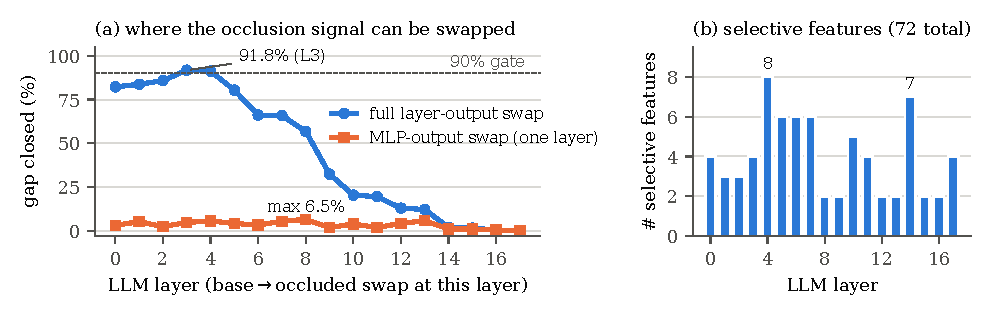
\includegraphics[width=\linewidth]{figures/fig_layer_profile.pdf}
  \caption{\textbf{Layer profile.} (a) Gap closed by replacing the base run's full layer output (blue) or only its MLP output (orange) with the occluded run's, at each layer (mean over 4 frames). (b) Number of occlusion-selective transcoder features per layer.}
  \label{fig:layers}
\end{figure}

\subsection{Q1: Occlusion-selective features exist}
Of 9,216 transcoder features, 72 (0.78\%) pass all three criteria, and every layer contributes 2--8 (Figure~\ref{fig:layers}b). Their median specificity is 0.64 (range 0.50--0.98) and median rise is 21.9 token-firings (range 1.4--127.8). Relative to their occlusion response, the median response to \cond{recolor} is 0.27, to \cond{absent} 0.11, and to \cond{slab\_miss} only 0.05. They are therefore bound to the object's location rather than to the paint itself. Spatially, the strongest layer-5 features fire on agentview tokens under the painted bowl and are silent there in every other condition (Appendix Figure~\ref{fig:contact}). Examples include L3~f76 (specificity 0.98), L5~f318 (0.96) and L15~f96 (rise 127.8). The top layers by summed score are 5, 0 and 4.

\subsection{Q2: The features are causal, but not sufficient}

\begin{table}[t]
\caption{\textbf{Goal 2: gap closed (\%) by patching base$\rightarrow$occluded} (all valid tokens; mean over 4 frames). ``Ceiling'' is the MLP-output swap at the same site(s). ``Margin'' is occlusion minus the stronger of the random and color controls; the pre-registered pass threshold is 10 points. $p$ is an exact one-sided paired sign-flip test of occlusion vs.\ random over frames; with 4 frames its minimum possible value is $1/16=0.0625$.}
\label{tab:goal2}
\centering\small
\resizebox{\linewidth}{!}{%
\begin{tabular}{@{}lrrrrrrr@{}}
\toprule
Site (\#features) & Occlusion & Random & Color & Ceiling & Occ./ceiling & Margin & $p$ \\
\midrule
Layer 0 (4)   & 0.18 & 0.27 & 0.37 & 3.09 & 6\% & $-0.2$ & 0.750 \\
Layer 4 (8)   & 1.17 & 0.20 & 0.25 & 5.55 & 21\% & $+0.9$ & 0.063 \\
Layer 5 (6)   & 1.92 & 0.27 & 0.46 & 4.15 & 46\% & $+1.5$ & 0.063 \\
Top-3 layers jointly (18) & 2.47 & -- & -- & -- & -- & -- & -- \\
All 18 layers (72) & \textbf{3.92} & 0.56 & 0.66 & 65.53 & 6\% & $+3.3$ & 0.125 \\
\midrule
All 18 layers, all 9,216 features & 40.14 & & & 65.53 & 61\% & & \\
\bottomrule
\end{tabular}}
\end{table}

\begin{figure}[t]
  \centering
  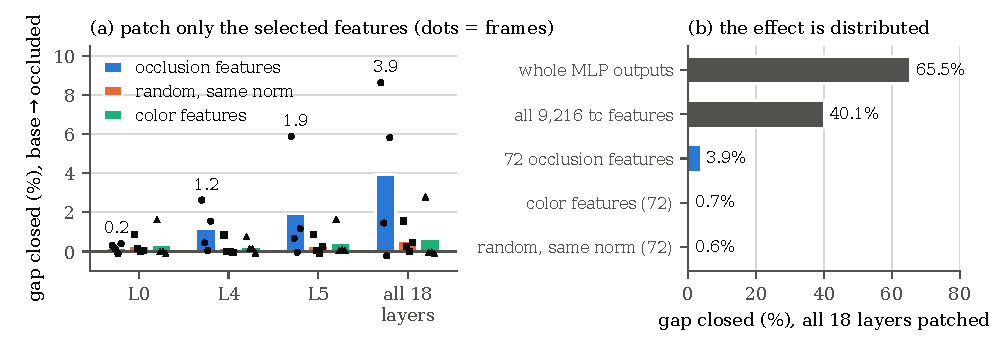
\includegraphics[width=\linewidth]{figures/fig_goal2_main.pdf}
  \caption{\textbf{Causal patching.} (a) Gap closed by patching only the selected occlusion features (blue), the same-norm random control (orange) and the color control (green), at single layers and at all 18 layers jointly. Dots are the four frames. (b) Decomposition at all 18 layers: the whole MLP outputs close 65.5\%, all transcoder features 40.1\%, the 72 occlusion features 3.9\%.}
  \label{fig:goal2}
\end{figure}

Table~\ref{tab:goal2} and Figure~\ref{fig:goal2} report the patching results.

\textbf{Above chance.} At layers 4 and 5 and at the all-layer site, occlusion features beat both controls. At all 18 layers jointly they close 3.92\% of the gap: $6.9\times$ the same-norm random sets (0.56\%) and $5.9\times$ the color set (0.66\%). They exceed every one of the 5 random draws in 3 of 4 frames (8.63 vs.\ at most 3.91; 1.45 vs.\ 0.87; 5.82 vs.\ 1.63). In the fourth frame (demonstration 1, $t{=}5$) they have no effect ($-0.23$), even though the MLP ceiling there is 83\%. The effect acts mainly through the target's tokens: patching only bowl tokens yields 3.08 points versus 0.96 for all other tokens. Single features are small: the largest is L5~f124 at 1.12 points. At layer 5 the single-feature effects sum to 3.0 points, more than the joint 1.9 (sub-additive).

\textbf{Not sufficient.} None of these margins approaches the pre-registered 10 points. The largest is $+3.3$ at the all-layer site. With four frames, even consistent wins give $p\ge0.0625$, so we treat the $\sim$6--7$\times$ ratios as suggestive. The size of the effect is what matters here:
\begin{itemize}[leftmargin=*,itemsep=0pt,topsep=1pt]
  \item Swapping all MLP outputs recovers 65.5\% of the gap, and all transcoder features together recover 40.1\% (61\% of that ceiling). The 72 selective features carry 9.8\% of what the transcoder features carry.
  \item In the remove direction, restoring base MLP outputs everywhere recovers 85.6\% of the way back to the base action, so MLP computation is largely necessary for the effect. Restoring only the occlusion features recovers 7.9\% (color: 3.0\%), and this is noisy across frames ($-3.9$ to $23.1$).
  \item The MLP ceiling itself is split 20.2\% on bowl tokens versus 29.4\% on other tokens.
\end{itemize}
Much of the MLP-mediated occlusion computation therefore happens away from the occluded patches, and most of it runs through features that are not occlusion-selective.

\textbf{Weak serial structure.} Injecting the layer-4 set activates 2.3\% of the layer-5 set's occlusion response (random: 0.04\%). The other edges are at most 0.8\%. The selected features form, at most, a weak chain.

\textbf{Q3 not run.} Because Q2 did not meet its criterion, the plan's gate stops before closed-loop evaluation. We report no success-rate numbers.

\section{Discussion}
\label{sec:discussion}

\paragraph{Report effects against the ceiling of the intervened site.} Check 4 validated the instrument with a \emph{residual} swap, which reaches 91.8\%. Transcoders, however, act on \emph{MLP} outputs, and a single MLP in \pifive{} carries at most 6.5\% of the occlusion effect. A plausible reason is that the image tokens already differ at the input embedding, and attention spreads that difference to every token whose keys and values the action expert reads, so no single MLP lies on a narrow path. A fixed absolute threshold at a single site is then unreachable \emph{by construction}. At layer 5, for example, the occlusion features recover 46\% of what the site can carry. We recommend reporting, for every VLA patching claim, the site's own ceiling next to the absolute effect. The all-layer site restores a meaningful ceiling (65.5\%). There the selective features recover only 6\% of it, which is the substantive negative finding.

\paragraph{What the features encode.} Our features respond to gray paint on the target and not to the same paint elsewhere. They also respond equally to paint with no object underneath: the correlation of $\Delta(\occ)$ and $\Delta(\cond{occluded\_absent})$ across the 72 features is 0.9986. This is expected. Because the paint covers the object, the two images differ in at most 0.39\% of pixels (the shadow ring), and in one frame they are identical. \pifive{} conditions on a single frame, so it cannot know what lies under the paint. The features are best described as ``uniform patch at the target location'' detectors. Object permanence in the developmental sense \citep{baillargeon1985object} requires temporal evidence that this protocol does not provide.

\paragraph{Why the effect is distributed.} The norm of the mean-centred MLP outputs grows by two orders of magnitude from early to late layers (RMS 36--60 in early layers, 9,375 at layer 17, consistent with massive activations \citep{sun2024massive}). Yet the residual-swap profile shows that the useful occlusion signal is available by the early-to-middle layers. The selective features are one small, interpretable slice of a broad change in many token representations. This is compatible with reports that vision pathways dominate action generation in \pifive{} \citep{grant2026features}. It adds that, at the level of MLP features, the occlusion signal is distributed rather than concentrated in a few concept features. The layer-level bottlenecks reported by \citet{shi2026vlatrace} concern attention routing, not feature sparsity, so the two findings are not in conflict.

\section{Limitations}
\label{sec:limitations}
\begin{itemize}[leftmargin=*,itemsep=1pt,topsep=2pt]
  \item \textbf{Scope and power.} We study one task and one object with four probe frames. Error bars are wide, and exact tests cannot reach conventional significance.
  \item \textbf{Frame selection.} Frames were selected for large gaps.
  \item \textbf{A synthetic occluder.} The occluder is a flat gray pixel patch, not a physical object. In the wrist camera it covers up to 22\% of the image.
  \item \textbf{No permanence contrast.} \cond{occluded\_absent} is nearly identical to \occ{} by construction, so the study cannot test object permanence.
  \item \textbf{Small transcoders.} They have 512 features and $k{=}16$ per layer and are trained on about 27k tokens from one scene. About 39\% of the MLP-mediated effect remains in their error terms.
  \item \textbf{Specificity-based selection.} Selecting features by attribution might find more causal sets.
  \item \textbf{A post-hoc site.} The all-layer site was added after the single-layer results were known. The criterion was not changed, and single-layer results are reported in full.
  \item \textbf{No closed-loop evaluation.} Q3 was not run.
\end{itemize}

\section{Conclusion}
We traced occlusion through the language backbone of a VLA policy with per-layer transcoders under a pre-registered, validated protocol. \pifive{} contains sparse features that selectively register a patch over the task's target object, and these features causally push the action toward its occluded counterpart more than matched controls do. They carry only a few percent of the effect, however. The occlusion signal is distributed across non-selective MLP features and across tokens beyond the occluded patches. For VLA interpretability, finding a selective feature is not the same as finding the mechanism, and causal claims should be stated relative to the ceiling of the intervened site.

\subsubsection*{AI use statement}
% AUTHORS: review and edit this statement so that it accurately reflects your process before submission.
Generative AI tools (a large language model assistant) were used to write and debug the experimental pipeline code (data rendering, hooks, transcoder training, patching), to compute the derived statistics, to produce the summary figures, and to draft this manuscript. The research question, the gated experimental plan and its thresholds were specified by the authors before the experiments were run. All reported numbers were cross-checked programmatically against the raw result files, and every cited work was checked against its public record. The authors reviewed all AI-assisted work and take full responsibility for the content of this paper.

\subsubsection*{Ethics statement}
This work analyzes a publicly released robot policy in simulation only. It involves no human subjects or personal data. Better understanding of how VLAs handle occluded objects could help identify unsafe failure modes before deployment.

\subsubsection*{Reproducibility statement}
Section~\ref{sec:method} and Appendix~\ref{app:repro} specify every hyper-parameter. The supplementary material contains the complete pipeline (one script with seven subcommands), the configuration, all 18 trained transcoders, the rendered probe frames, every raw result file (including the 736 individual patching runs), and the scripts that regenerate all derived statistics and figures in this paper.

\bibliography{references}
\bibliographystyle{iclr2027_conference}

\appendix
\section{Reproducibility details}
\label{app:repro}
\paragraph{Software and hardware.} We used LeRobot 0.6.1, transformers 5.5.4, PyTorch 2.11.0 (CUDA 12.8), MuJoCo 3.8.1, robosuite 1.4.0, NumPy 2.2.6 and Python 3.12, on one NVIDIA A100-SXM4-80GB. Wall-clock times per step were: policy load 149\,s (repeated for each step), frames 205\,s, validation 285\,s, activation capture 201\,s, transcoder training 375\,s, Goal 1 10\,s, and Goal 2 688\,s.

\paragraph{Implementation notes.}
\begin{itemize}[leftmargin=*,itemsep=0pt,topsep=1pt]
  \item The checkpoint enables \texttt{torch.compile} in max-autotune mode, whose CUDA graphs reuse output buffers and bypass Python hooks. We disable it.
  \item robosuite 1.4's segmentation readout overflows under NumPy 2, so we decode MuJoCo segmentation buffers ourselves.
  \item The target object is resolved from the task's BDDL.
  \item Transcoder training uses a learning-rate warm-up over the first 5\% of steps and a linear decay over the last 20\%. Dead features are those that have not fired for 50 steps.
  \item Bowl tokens are the SigLIP patches (a $16\times16$ grid per image, after the LIBERO $180^\circ$ image flip) whose area is at least 10\% covered by the painted region.
\end{itemize}

\paragraph{Deviations from the written plan.}
\begin{itemize}[leftmargin=*,itemsep=0pt,topsep=1pt]
  \item The plan assumed 32 LLM layers; \pifive{}'s Gemma-2B backbone has 18.
  \item The plan named 400 transcoder steps; we used 3,000 after the 400-step run missed Check 5 (median FVU 0.209 vs.\ 0.20).
  \item The all-layer Goal 2 site was added after the single-layer run.
  \item Closed-loop Goal 3 was gated off.
\end{itemize}

\section{Per-frame and per-layer results}
\begin{table}[h]
\caption{Per-frame action gaps (normalized RMSE vs.\ \cond{base}) under each condition, and the RMSE from changing only the sampling noise.}
\centering\small
\resizebox{\linewidth}{!}{%
\begin{tabular}{@{}lrrrrrrr@{}}
\toprule
Frame (demo, $t$) & \occ & \cond{absent} & \cond{recolor} & \cond{slab\_miss} & \cond{occ\_absent} & noise & gap/noise \\
\midrule
0 (0, 35) & 0.520 & 1.060 & 0.229 & 0.337 & 0.504 & 0.127 & 4.1 \\
1 (0, 41) & 0.516 & 0.922 & 0.127 & 0.112 & 0.545 & 0.138 & 3.7 \\
2 (1, 5)  & 0.666 & 0.967 & 0.392 & 0.089 & 0.666 & 0.151 & 4.4 \\
3 (1, 32) & 0.522 & 0.831 & 0.074 & 0.111 & 0.493 & 0.178 & 2.9 \\
\bottomrule
\end{tabular}}
\end{table}

\begin{table}[h]
\caption{Per-layer transcoder quality and single-layer ceilings (mean over 4 frames).}
\centering\small
\setlength{\tabcolsep}{3.2pt}
\resizebox{\linewidth}{!}{%
\begin{tabular}{@{}l*{18}{r}@{}}
\toprule
Layer & 0 & 1 & 2 & 3 & 4 & 5 & 6 & 7 & 8 & 9 & 10 & 11 & 12 & 13 & 14 & 15 & 16 & 17 \\
\midrule
FVU (held-out) & .018 & .149 & .158 & .171 & .163 & .156 & .198 & .152 & .202 & .199 & .258 & .199 & .233 & .188 & .182 & .177 & .022 & .076 \\
Splice / gap & .070 & .099 & .071 & .101 & .092 & .118 & .108 & .110 & .132 & .077 & .118 & .124 & .136 & .161 & .090 & .078 & .010 & .000 \\
Full swap (\%) & 82.3 & 83.8 & 85.8 & 91.8 & 91.3 & 80.4 & 66.2 & 65.9 & 56.8 & 32.4 & 20.4 & 19.5 & 12.9 & 12.1 & 1.8 & 1.5 & 0.4 & 0.0 \\
MLP swap (\%) & 3.1 & 5.2 & 2.4 & 4.7 & 5.6 & 4.1 & 3.2 & 5.4 & 6.5 & 1.8 & 3.9 & 1.8 & 4.2 & 5.7 & 1.0 & 1.0 & 0.4 & 0.0 \\
\# selective & 4 & 3 & 3 & 4 & 8 & 6 & 6 & 6 & 2 & 2 & 5 & 4 & 2 & 2 & 7 & 2 & 2 & 4 \\
\bottomrule
\end{tabular}}
\end{table}

\begin{table}[h]
\caption{All-layer site, per frame (gap closed, \%; inject unless stated).}
\centering\small
\begin{tabular}{@{}lrrrrr@{}}
\toprule
Method & Frame 0 & Frame 1 & Frame 2 & Frame 3 & Mean \\
\midrule
Occlusion features (72) & 8.63 & 1.45 & $-0.23$ & 5.82 & 3.92 \\
Random, same norm (mean of 5) & 1.56 & 0.26 & 0.00 & 0.45 & 0.56 \\
Color features (72) & 2.79 & $-0.04$ & $-0.03$ & $-0.10$ & 0.66 \\
All transcoder features & 32.25 & 16.00 & 62.67 & 49.65 & 40.14 \\
MLP swap (ceiling) & 76.58 & 30.22 & 83.04 & 72.28 & 65.53 \\
Occlusion features, remove & 13.18 & $-3.88$ & $-0.69$ & 23.07 & 7.92 \\
MLP swap, remove & 66.20 & 88.72 & 93.51 & 93.96 & 85.60 \\
\bottomrule
\end{tabular}
\end{table}

\section{Additional figures}
\begin{figure}[h]
  \centering
  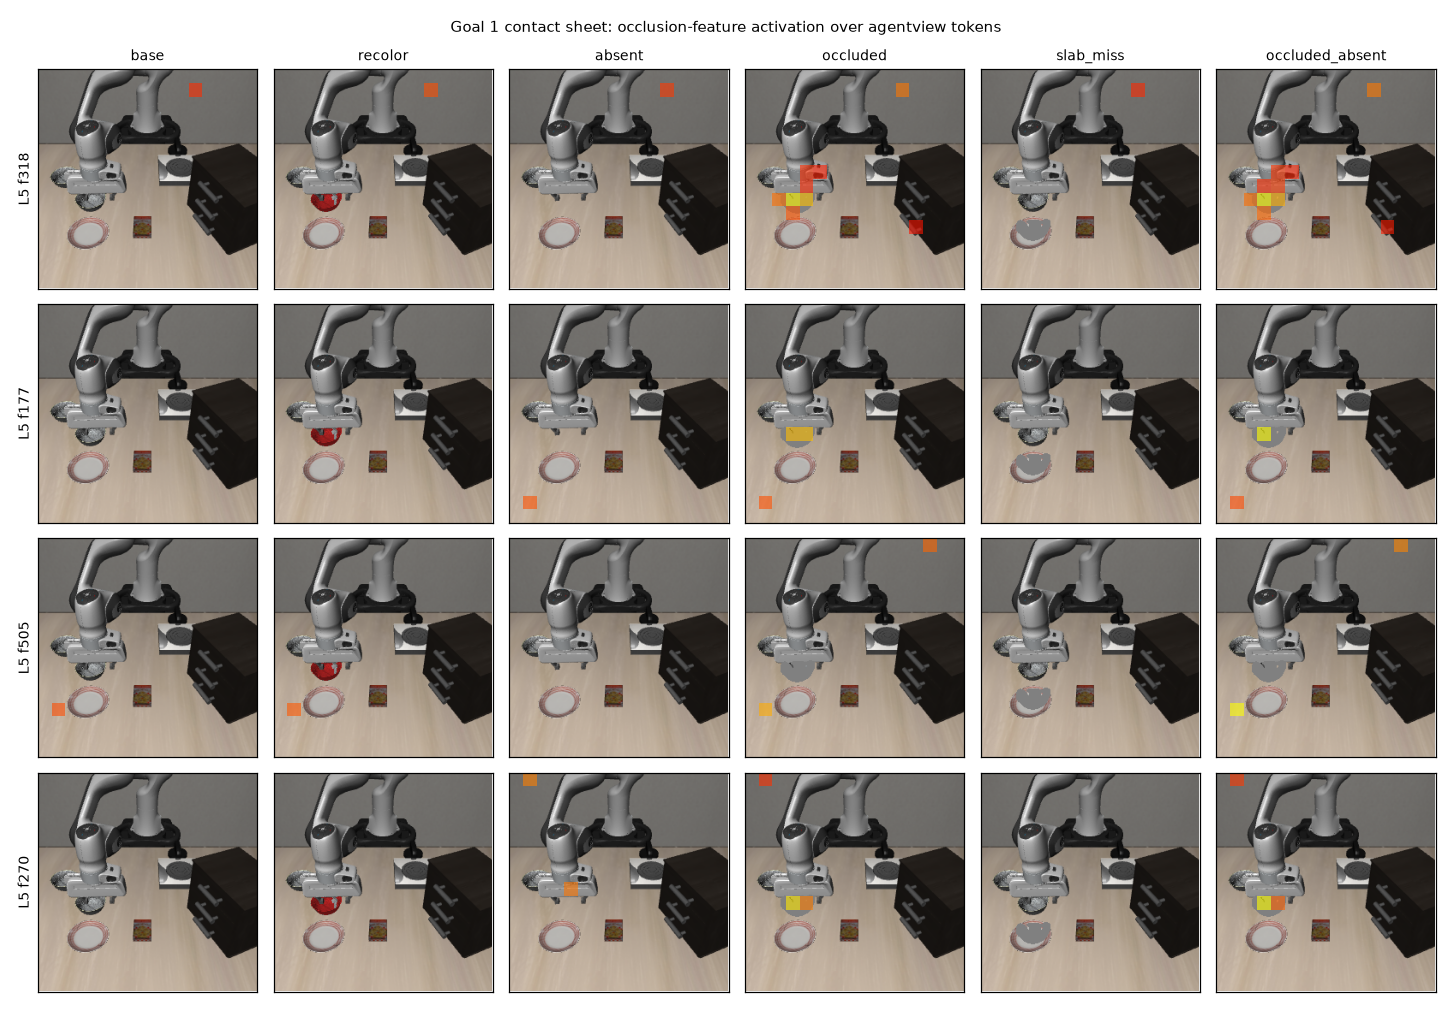
\includegraphics[width=0.92\linewidth]{figures/fig_goal1_contact_sheet.png}
  \caption{Activation maps of the four strongest layer-5 occlusion features over agentview tokens (frame 0), for every condition. The features fire under the painted bowl and are silent there when the bowl is visible, recolored, removed, or when the paint is elsewhere. They fire equally under \cond{occluded\_absent}.}
  \label{fig:contact}
\end{figure}

\begin{figure}[h]
  \centering
  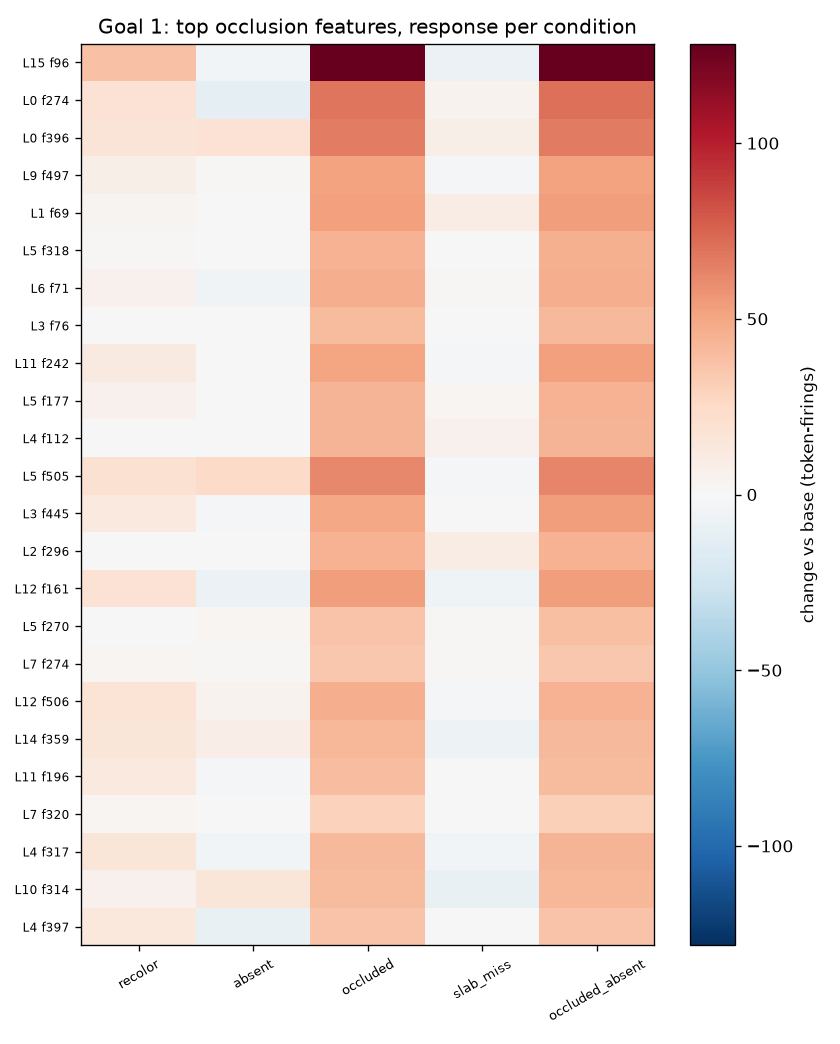
\includegraphics[width=0.55\linewidth]{figures/fig_goal1_features.png}
  \caption{Response of the 24 highest-scoring occlusion features to each condition (change vs.\ \cond{base}, in token-firings). The \occ{} and \cond{occluded\_absent} columns are nearly identical.}
\end{figure}

\begin{figure}[h]
  \centering
  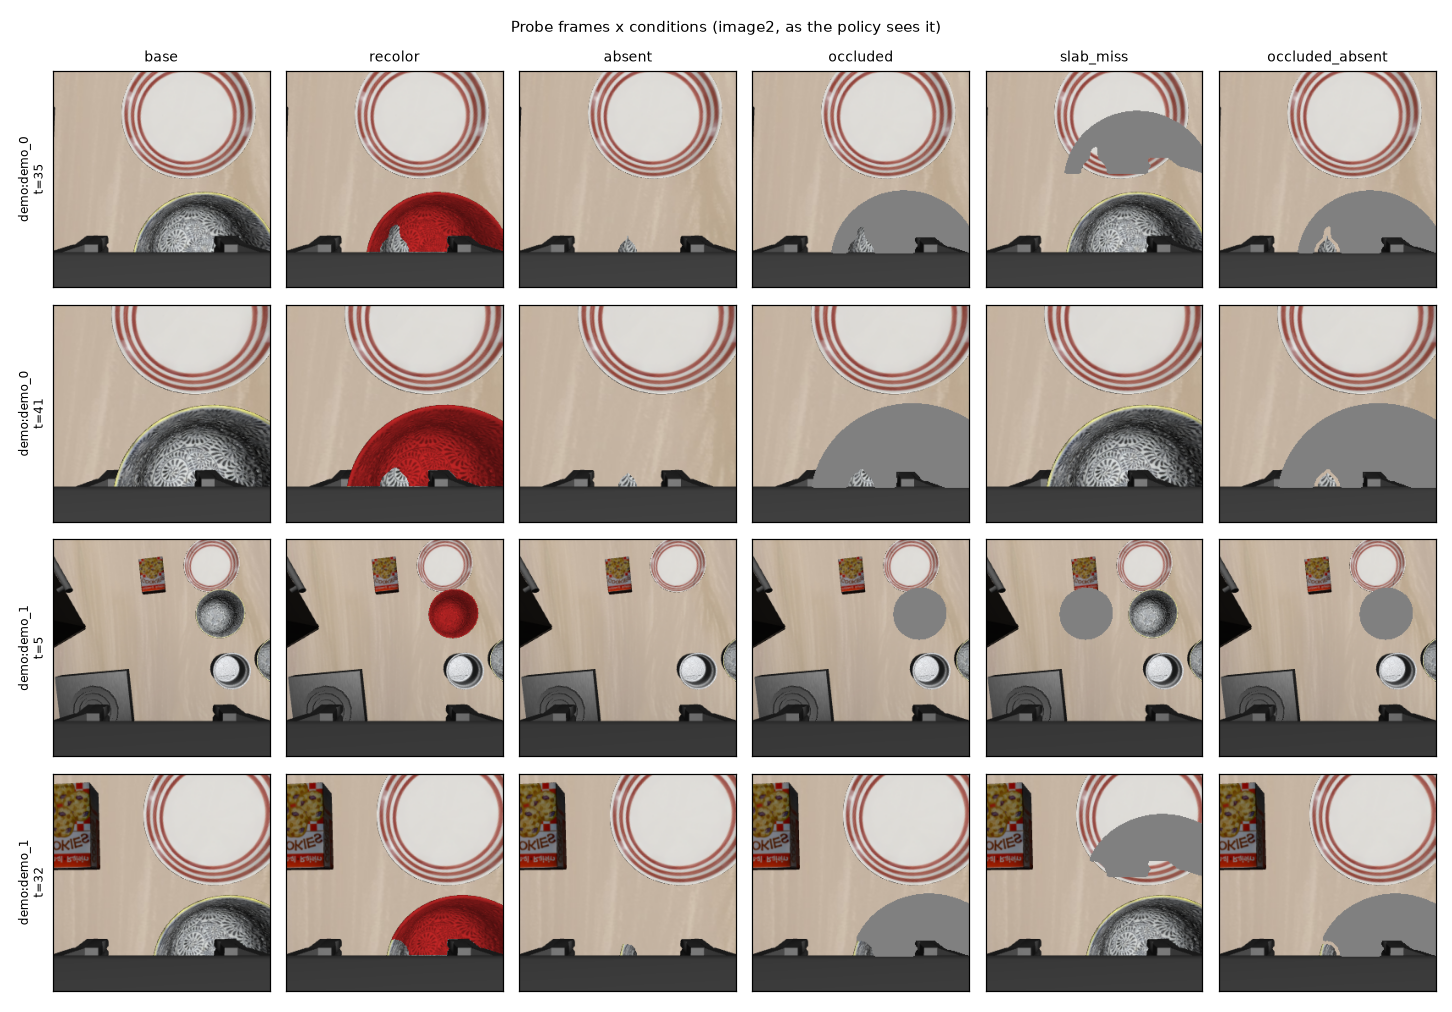
\includegraphics[width=0.92\linewidth]{figures/fig_probe_conditions_wrist.png}
  \caption{All four probe frames in the wrist camera. In frame 1 there was no room for the off-target patch (\cond{slab\_miss}), so the wrist image is unedited in that condition. In frames 0 and 3 the off-target patch partly covers the plate.}
\end{figure}

\end{document}
